%!TEX root = /Users/dbreuer/Documents/Work/_FH/_Master/master_thesis/Main/Master Thesis.tex

\chapter{COSIMA - Eine dienstorientierten Multimediaarchitektur} % (fold)
\label{cha:eine_dienstorientierten_multimediaarchitektur}

  Im Abschnitt~\ref{sec:motivation} wurde bereits kurz darauf eingegangen, dass die vorliegenden Arbeit vor dem Hintergrund des COSIMA-Projekts entstanden ist. In diesem Kapitel soll dieses Projekt so weit vorgestellt werden, dass für den weiteren Verlauf der Arbeit ein grundlegendes Verständnis über die Ziele, Alleinstellungsmerkmale und Herausforderungen existiert.
  
\section{Motivation und Ziele von COSIMA} % (fold)
\label{sec:motivation_und_ziele_von_cosima}

  Das COSIMA-Projekt ist aus dem Wahlpflichtfach Modellierung in audio-visuellen Medien (MIAV\abk{MIAV}{Modellierung in audio-visuellen Medien}) an der Fachhochschule Köln im Masterstudiengang der Medieninformatik hervorgegangen. Im Rahmen einer Projektarbeit wurde das die Projektidee weiter ausgearbeitet und konzeptioniert. Die Ergebnisse dieser Arbeit wurden als Institutsbericht an Fachhochschule Köln bereitsgestellt und sind dort im Detail einsehbar~\citep{bericht}.
  
  Das folgende Kapitel wird daher nur auf die wesentliche Punkte des COSIMA-Projekts eingehen und ihre Relevanz für diese Arbeit herausstellen. Die ursprüngliche Idee hinter COSIMA war es ein Framework zu entwickeln, dass die Entwicklung von Multimediaanwendungen vereinfacht. Im Gegensatz zu anderen Medienframeworks, wie etwa dem \emph{Java Media Framework} (JMF\abk{JMF}{Java Media Framework}), wurde bei dem COSIMA-Projekt ein ganzheitlicher Ansatz verfolgt.
  
  Im Institutsbericht wird darauf hingewiesen, "`dass die Entwicklung von Multimediaanwendungen derzeit verhältnismässig aufwendig ist"'~\citep[S. 2]{bericht}. Eine Ursache dieser Problematik, liegt nach Aussage der Autoren darin begründet, dass sich die zur Zeit verfügbaren Rahmenwerke im Bereich der Multimediaverarbeitung auf einen sehr engen Einsatzbereich beschränken. Neben JMF sind hier zusätzlich noch \emph{QuickTime}\footnote{\url{http://www.apple.com/quicktime/}} und \emph{ImageJ}\footnote{\url{http://rsbweb.nih.gov/ij/}} zu nennen. Andere Aspekte von Multimediaanwendungen, wie etwa die Integration von Metadaten, müssten von dem Anwendungsentwickler erst manuell mit diesen Rahmenwerken integriert werden. "`Ein Meta-Framework, welches die bestehenden Ansätze verbinden und integrieren könnte, würde die Wiederverwendbarkeit und generelle Entwicklungsarbeit positiv beeinflussen, beziehungsweise vereinfachen"'~\citep[S. 3]{bericht}, wird von den Autoren des Berichts daher als Bestreben hinter dem COSIMA-Projekt angeführt.
  
  Neben der Notwendigkeit ein \emph{Meta-Framework}\footnote{Das ursprüngliche Ziel war tatsächlich ein Framework zu schaffen. Erst während der Validierung im Rahmen dieser Arbeit ist zu Tage gekommen, dass es sich mehr um eine Architektur handelt und weniger um ein Framework. Im weiteren Verlauf wird darauf jedoch noch genauer eingegangen.} zu schaffen, führen die Autoren als weiteren Beweggrund das Fehlen einer Architektur für Multimediaanwendungen an. Innerhalb dieser Architektur könnten sich Anwendungsentwickler wesentlicher effektiver bewegen und müssten nicht erst eine eigene Architektur von Grund auf entwerfen.
  
  Da sich mit den meisten bestehenden Multimedia-Rahmenwerke keine verteilten Anwendungen realisieren lassen, lag auch dieser Aspekt von Beginn an im Fokus der Konzeptionierung. Als Grundlage eine geeignete Architektur zu konzeptionieren, die es ermöglicht, verteilte Anwendungen zu realisieren, diente das Konzept der \emph{Service-oriented Architecture} (SOA\abk{SOA}{Service-oriented Architecture}) oder \emph{Dienst-orientierten Architektur}.
  
  Die hier aufgeführten Punkte haben initial die Entwicklung eines Rahmenwerkes motiviert, dass später im COSIMA-Projekt aufgehen sollte. Die im Verlauf der Projektarbeit entwickelten Ziele von COSIMA sind im nächsten Abschnitt zusammen gefasst.
  
\subsection{Ziele} % (fold)
\label{sub:ziele}

  Das \emph{Mission Statement} des COSIMA-Projekts fasst alle Ziele des Projekts in einer Kernaussage zusammen:

  \begin{quote}
    \emph{``MIAV ist ein integratives, komponentenbasiertes Meta-Framework mit gezielter Ausrichtung auf Multimediaverarbeitung. Es vereinfacht die Entwicklung von verteilten Multimedia-Applikationen durch eine flexible, dienst-orientierte Architektur. Die Wiederverwendbarkeit von Komponenten und bestehenden Frameworks wird dadurch begünstigt.''} (aus~\citep[S. 2]{bericht})\footnote{Die Bezeichnung "`COSIMA"' hat das Projekt erst nach Fertigstellung des Berichts erhalten, daher findest sich hier noch die zuvor verwandte provisorische Bezeichnung \emph{MIAV-Framework}.}
  \end{quote}

  Neben den zentralen Aspekten \emph{dienst-orientierte Architektur}, \emph{Integration} und \emph{Meta-Framework}, die im Abschnitt zuvor bereits dargestellt wurden, nennen die Autoren hier zusätzlich noch die Aspekte der \emph{komponentenbasierten Architektur}, \emph{Wiederverwendbarkeit} und natürlich der \emph{Medienverarbeitung}.
  
  Neben den hier genannten Zielen, die das COSIMA-Projekt zu erreichen versucht, zeichnet sich das Projekt durch seine spezifischen Charakteristika in Bezug auf andere Multimedia-Rahmenwerke aus. Diese Alleinstellungsmerkmale werden im nächsten Abschnitt genauer betrachtet.

  % - Welche Ziele verfolgt das COSIMA-Projekt?
  % - Warum handelt es sich um eine Architektur und nicht um ein Framework!!!! (Im Bericht noch anders, irgendwie muss das hier verwurstet werden!)
  % - Weiterentwicklung der Definition seit dem Bericht

% subsection ziele (end)
  
% section motivation_und_ziele_von_cosima (end)

\section{Alleinstellungsmerkmale} % (fold)
\label{sec:alleinstellungsmerkmale}

  Aus den in Abschnitt~\ref{sub:ziele} dargestellten Zielen des COSIMA-Projekts lassen sich die folgenden Merkmale extrahieren, die COSIMA im Bereich der Multimedia-Rahmenwerke und -Anwendungen einmalig machen~\citep[S. 3f]{bericht}:
  
  \begin{description}
    \item[Verteiltheit] COSIMA ist konzeptioniert als ein verteiltes System.
    \item[Dienstorientierung] Angelehnt an die \emph{Service-Oriented Architecture} (SOA), sind die Bausteine in COSIMA als Dienste modelliert.
    \item[Integration] Bestehende Frameworks können in Form von Diensten angeboten und so ihre Funktionalität eingebunden werden.
    \item[Erweiterbarkeit] Die Dienstorientierung erlaubt die Einbindung eigener Komponenten.
    \item[Skalierbarkeit] In einer verteilten, dezentralisierten Umgebung können einzelne Funktionalitäten als Dienste völlig unabhängig voneinander betrieben werden. Die Folge ist die vollständige Flexibilität in Bezug auf die Skalierbarkeit des gesamten Systems~\citep[S. 294]{web_services_principles_and_technology}.
    \item[Medienobjekt-Modellierung] Modellierung von Medien in ganzheitlicher Betrachtungsweise von Rohdaten und Metadaten in einem Objekt.
    \item[Meta-Ebene] COSIMA fokussiert nicht auf Datensicht oder Metadatensicht sondern abstrahiert auf höhere Ebene.
    \item[Medienverarbeitung] Ganzheitliche Sicht auf Medienverarbeitung: Produktion, Verarbeitung, Transformation, Anreicherung, Wiedergabe, Ausgabe von Daten und Metadaten.
    \item[Architektur] COSIMA stellt eine Architektur für Multimediaanwendungen.
  \end{description}
  
  Basierend auf den vorgestellten Zielen und Alleinstellungsmerkmalen wurde die Architektur entworfen, die in dieser Arbeit validiert und prototypisch realisiert wurde. Im Folgenden Abschnitt wird diese Architektur im Detail vorgestellt werden.

% section alleinstellungsmerkmale (end)

\section{Architektur} % (fold)
\label{sec:architektur}

  Die Architektur des COSIMA-Projekts ist iterativ in einem dedizierten Vorgehen\footnote{Dieses Vorgehen wird detailliert im Institutsbericht vorgestellt. Eine Erläuterung in diesem Rahmen ist nicht angemessen und wird daher ausgelassen.} bis zu dem Punkt entwickelt worden, der als Ausgangspunkt für die Betrachtungen in dieser Arbeit dient.

\subsection{Einführung} % (fold)
\label{sub:einfuehrung}

  Bei der Konzeption und Entwicklung der Architektur sind unterschiedliche Sichten auf diese erstellt worden. Diese Sichten entsprechen denen von Starke in~\citep[S. 83]{effektive_software_architekturen} beschriebenen vier Arten von Sichten auf eine Software-Architektur: \emph{Kontextsichten}, \emph{Bausteinsichten}, \emph{Laufzeitsichten} und \emph{Verteilungssichten}.

  Für das COSIMA-Projekt wurden bisher Darstellungen aus zwei dieser Kategorien erstellt: eine der Kontextsichten und drei der Bausteinsichten. Die Kontextsichten legen laut Starke den "`Fokus auf den Zusammenhang oder das Umfeld des Systems"'~\citep[S. 87]{effektive_software_architekturen}, was auch auf die in Abbildung~\ref{fig:images_Kontextsicht_Architektur_COSIMA} dargestellte Kontextsicht von COSIMA zutrifft. Hier wird lediglich ein abstrakter und vor allem nicht formaler Überblick über die Architektur und beteiligte Systeme gegeben. Die Darstellungen, die sich den Bausteinsichten zuordnen lassen, sind namentlich das \emph{Komponentendiagramm}, das \emph{Kompositionsstrukturdiagramm} und der \emph{Grobentwurf} der Architektur. Diese finden sich jeweils in~\citep{bericht} und sollen an dieser Stelle nicht weiter betrachtet werden\footnote{\textbf{TODO}: Im weiteren Verlauf werden sicher Teile aus diesen Diagrammen benötigt, daher muss dann darauf referenziert werden.}. Für die weitere Vorstellung der Architektur soll an dieser Stelle die Kontextsicht genügen.

\begin{figure}[ht]
  \centering
    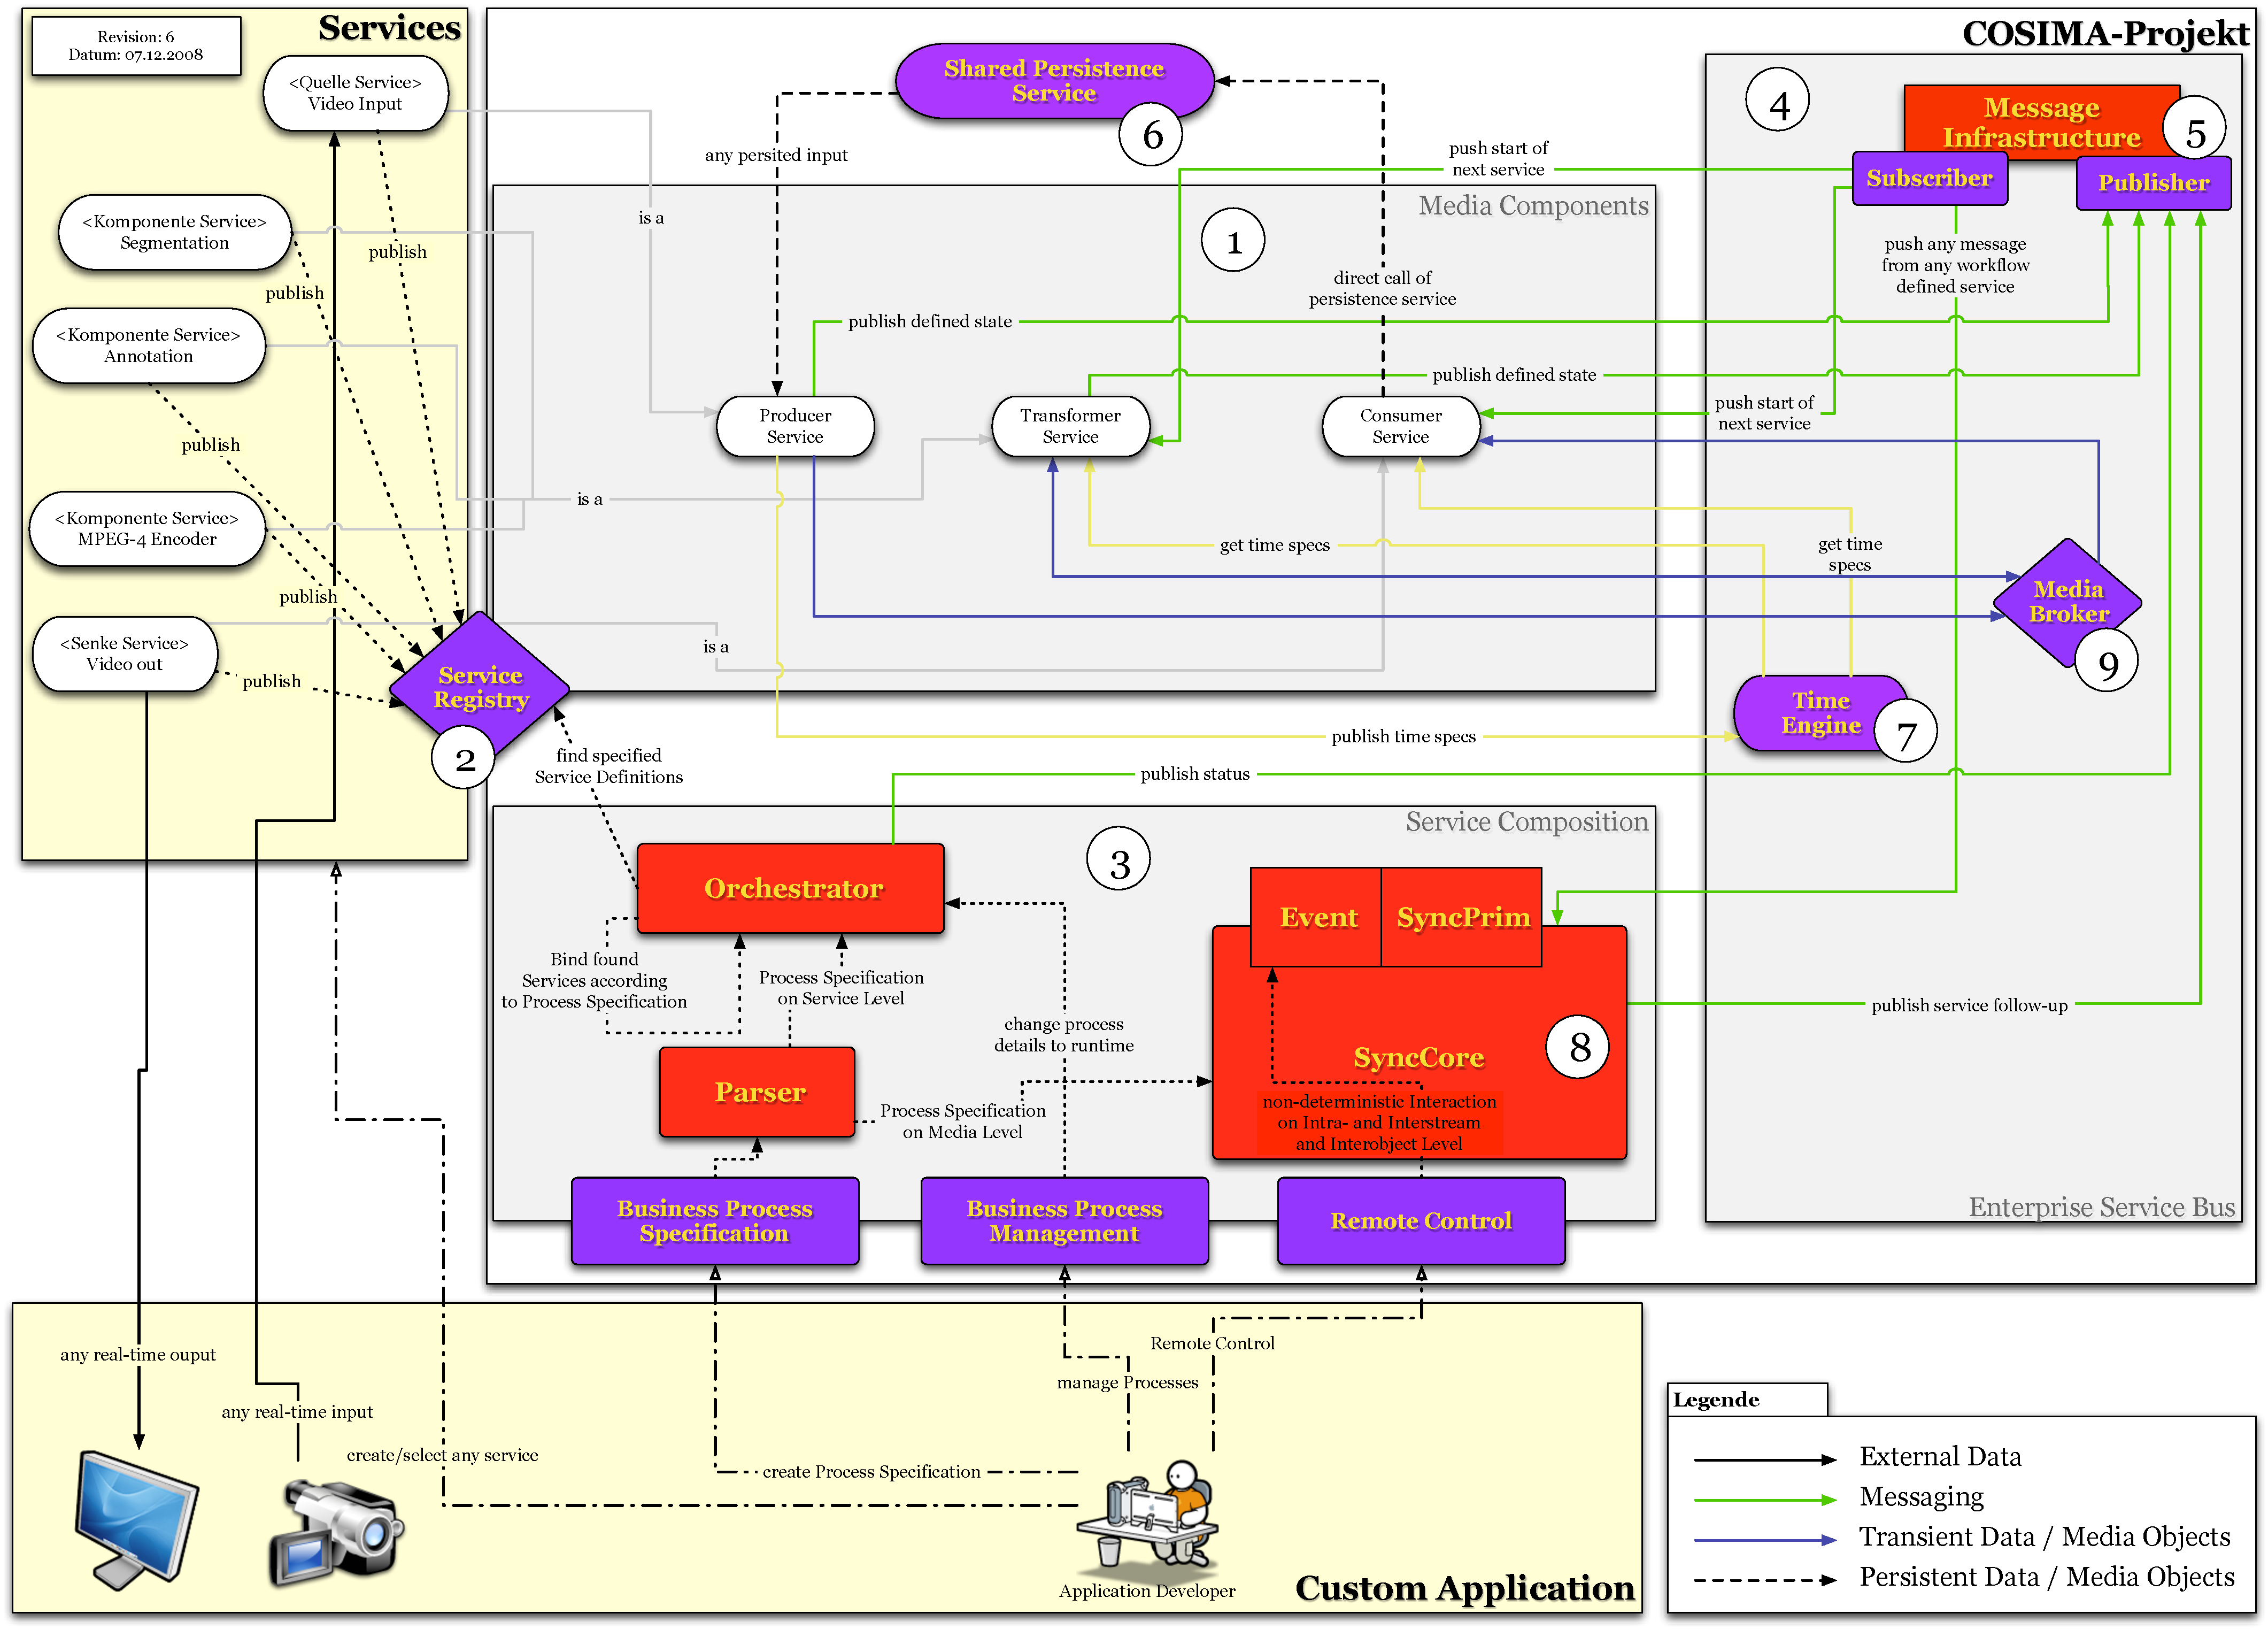
\includegraphics[width=.9\textwidth]{images/Kontextsicht_Architektur_COSIMA}
  \caption{Kontextsicht der Architektur des COSIMA-Projekts}
  \label{fig:images_Kontextsicht_Architektur_COSIMA}
\end{figure}

  In der späteren prototypischen Realisierung und anschließenden Validierung der Architektur sollen und können nur Fragmente der Architektur umgesetzt werden, daher ist es sehr wichtig, solche Fragmente zu wählen, die für eine Weiterentwicklung von besonderem Interesse sind. Im Folgenden werden daher die zentralen Komponenten des COSIMA-Projekts kurz vorgestellt. \emph{Später soll dann eine Auswahl getroffen werden.}

  % - Kernpunkte der Architektur herausarbeiten
  % - Diese Kernpunkte müssen in der Realisierung/Validierung entsprechend besondere Berücksichtigung finden

% subsection einfuehrung (end)

\subsection{Medienverarbeitende Komponenten} % (fold)
\label{sub:medienverarbeitende_komponenten}

  Den Kern von COSIMA machen die medienverarbeitenden Komponenten aus, die vom Anwendungsentwickler in eine entsprechende Abfolge gebracht werden und damit die später Multimediaanwendung selbst darstellen: \emph{Producer}, \emph{Transformer} und \emph{Consumer}. Dem Entwurf der Komponenten liegt das \emph{Quelle-Komponente-Senke} Prinzip zu Grunde. Die innerhalb des COSIMA-Projekts verwendete Bezeichnung ist nach~\citep{a_multimedia_component_kit,multimedia_component_frameworks} ebenso valide wie die geläufigere Bezeichnung "`Quelle-Komponente-Senke"'. Da es sich bei COSIMA jedoch um eine komponentenbasierte Architektur handelt, wodurch Benennungsschwierigkeiten aufkamen, die die Verwendung einer alternativen Begrifflichkeit begünstigten.
  
  Diese medienverarbeitenden Komponenten sind alle als Dienste ausgeprägt, um dem Anspruch der Dienstorientierung gerecht zu werden. Eine Komponente kann dabei niemals eine andere Komponente direkt aufrufen, diese Aufgabe obliegt der \emph{Service Komposition} (siehe Abschnitt~\ref{sub:service_komposition}). Jede dieser Komponenten muss sich dazu bei seiner Initiierung beim Service Repository registrieren, der in~\ref{sub:service_registry} näher beschrieben wird.
  
  Der Austausch der zu verarbeitenden Medien zwischen den einzelnen Komponenten geschieht auschließlich über den \emph{Media Broker}, der unter~\ref{sub:medienobjekt} weiter ausgeführt wird. Ein genereller Nachrichtenaustausch unter den Komponenten im speziellen und mit den restlichen Elementen der Architektur wird über das Nachrichtensystem (\ref{ssub:nachrichtensystem}) realisiert. Persistenz von Daten und die Synchronisation werden von einem \emph{Persistence Data Service} bzw. der \emph{Timing Engine} übernommen. Beide Komponenten werden in~\ref{sub:infrastruktur} näher beschrieben. Teile dieser Architekturelemente sollen einmal in einem Service Bus aufgehen~\citep[S. 18]{bericht}.

% subsection medienverarbeitende_komponenten (end)

\subsection{Service Registry} % (fold)
\label{sub:service_registry}

  Die Service Registry ist nach~\citep{service_oriented_computing}, als konstituierendes Element innerhalb einer SOA, selbst wieder ein Dienst, der die Dienstbeschreibungen anderer Dienste vorhält und bereitstellt. Jeder Dienst innerhalb von COSIMA muss daher seine Beschreibung bei der Service Registry bekannt machen. Es kann demnach auch keinen anderen Weg geben als über die Service Registry eine Verbindung zu einem Service aufzunehmen.

  % - Zentrale Stelle zur Registrierung/Auffindung von Services
  % - Definition der allgemeinen Schnittstelle für COSIMA-Services

% subsection service_registry (end)

\subsection{Servicekomposition} % (fold)
\label{sub:service_komposition}

  Abbildung \ref{fig:images_Basic_SOA} zeigt die einfachste Form einer dienstorientierten Architektur, wie sie im Rahmen des Paradigmas des \emph{Service Oriented Computing} (SOC\abk{SOC}{Service Oriented Computing}) vorgestellt wurde~\citep{service_oriented_computing}. Wie bereits im Abschnitt \ref{sub:service_registry} gesagt wurde, muss ein Dienst selbstständig bei der Service Registry nach der Beschreibung eines anderen Dienstes fragen, um diesen dann ansprechen zu können. Dieses Vorgehen wirkt sich jedoch negativ auf die Kopplung einzelner Dienste aus; Die Kopplung der Dienste wird also größer.
  
\begin{figure}[hb]
  \centering
    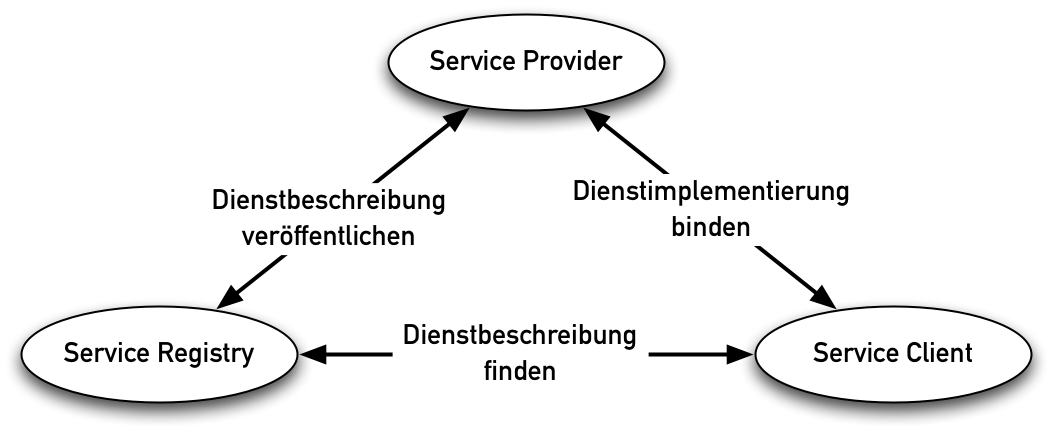
\includegraphics[width=.9\textwidth]{images/Basic_SOA.png}
  \caption{Einfachste Form einer dienstorientierten Architektur (nach~\citep{service_oriented_computing})}
  \label{fig:images_Basic_SOA}
\end{figure}

  In einer dienstorientierten Architektur wird aber voraus gesetzt, dass die einzelnen Dienste möglichst lose gekoppelt sind~\citep[S. 162]{soa_goes_real}. Um diese Kopplung zwischen den Dienste aufzubrechen, kann die Information welche Dienste miteinander interagieren sollen, in Form der \emph{Servicekomposition} externalisiert werden.

  Durch die Servicekomposition kreieren Entwickler Applikationen innerhalb von dienstorientierten Architekturen. Die Servicekomposition setzt dabei auf die grundlegenden Elemente einer SOA auf~\citep[S. 51]{milanovic2004csw} und stellt damit ein zentrales Element dar, um überhaupt aus einer Reihe von einzelnen Diensten eine Applikation zu aggregieren.
  
  Nach~\citep[S. 104]{masak2007ssb} kann die Servicekomposition dabei aus zwei unterschiedlichen Perspektiven betrachtet werden: der \emph{Geschäftsprozesskomposition} und der \emph{Servicelevelkomposition}. Bei der Geschäftsprozesskomposition werden "`völlig neue Geschäftsprozesse aus bestehenden Teilprozessen oder Services"' (\citep[S. 104]{masak2007ssb}) komponiert. Eine Einbettung in eine Organisation steht hier klar im Vordergrund. Bei der Servicelevelkomposition steht vielmehr "`die Interoperabilität und technische Machbarkeit im Vordergrund"' (\citep[S. 105]{masak2007ssb}) und es wird keine Rücksicht auf eine mögliche Organisationstruktur genommen. Da eines der Ziele von COSIMA die Entwicklung von Multimedia-Applikationen ist (vgl. Abschnitt \ref{sub:ziele}) und nicht die Abbildung von Geschäftsprozessen im Vordergrund steht, wird dieser Aspekt in dieser Arbeit nicht weiter verfolgt.
  
\subsubsection{Kompositionsarten} % (fold)
\label{ssub:kompositionsarten}

  Bei der Komposition von Diensten werden in der Literatur unterschiedliche Arten unterschieden. Die beiden grundsätzlichen, für COSIMA relevanten, werden bei Papazoglou in~\citep[S. 41]{papazoglou2007soc} genannt: \emph{Orchestrierung} und \emph{Choreographie}. Im Folgenden sollen diese beiden Ansätze genauer betrachtet werden.
  
\paragraph{Orchestrierung} % (fold)
\label{par:orchestrierung}
  
  Orchestrierung wird von Papazoglou wie folgt definiert:
  
  \begin{quote}
    \emph{"`Orchestration describes how services interact at the message level, including the business logic and execution order of interactions under control of a single end point. It is an executable business process that can result in a long-lived, transactional, multistep process model."'} (\citep[S. 41]{papazoglou2007soc})
  \end{quote}
  
  Wesentlich sind also die Interaktionen verschiedener Dienste, die von einer zentralen Stelle über einen Nachrichtenaustausch koordiniert und kontrolliert werden. Des Weiteren ist das Ergebnis ein ausführbarer Geschäftsprozess.

% paragraph orchestrierung (end)

\paragraph{Choreographie} % (fold)
\label{par:choreographie}

  In der Definition von~\citep{peltz2003wso} wird der Unterschied zwischen Choreographie und Orchestrierung deutlich:
  
  \begin{quote}
    \emph{"`[...] choreography, which is more collaborative and allows each involved party to describe its part in the interaction. Choreography tracks the message sequences among multiple parties and sources --- typically the public message exchanges that occur between Web services --- rather than a specific business process that a single party executes."'} (\citep[S. 46]{peltz2003wso})
  \end{quote}

  Choreographie verfolgt also einen dezentralen Ansatz; Es gibt nicht eine Instanz, die den Nachrichtenfluss kontrolliert, vielmehr tritt der Nachrichtenfluss zwischen den einzelnen Diensten in den Vordergrund.
  
  Bei der Betrachtung beider Ansätze wird deutlich, dass die Trennung von Choreographie und Orchestrierung eher künstlich erscheint und man stimmt bereits darüber überein, dass sie beide in einer Sprache und Umgebung\footnote{Zur Umsetzung dieser beiden Kompositionsansätze existieren zahlreiche, unterschiedliche Technologien und (Sprach-)Standards, deren weitere Betrachtung nicht mehr Teil dieser Arbeit sein kann.} vereint werden sollten~\citep[S. 42]{papazoglou2007soc}.

% paragraph choreographie (end)

% subsubsection kompositionsarten (end)

\subsubsection{Relevanz fuer COSIMA} % (fold)
\label{ssub:relevanz_fuer_cosima_komposition}

  Es wurde deutlich, dass die Servicekomposition für eine dienstorientierte Architektur von elementarer Bedeutung ist. Jedoch wurde auch klar, dass die Servicekomposition in COSIMA noch nicht so verstanden wird, wie sie in der Literatur verstanden wird; Dort findet eine Betrachtung im Kontext von Geschäftsprozessen statt. Sowohl in der bisherigen Zieldefinition von COSIMA, als auch in dem Szenario für die prototypische Realisierung der Architektur, dass in Kapitel~\ref{cha:szenario} vorgestellt wird, liegt der Fokus jedoch nicht auf Geschäftsprozessen. Daher ist auch eine weitere Betrachtung der genannten Details für diese Arbeit nicht notwendig. Dennoch kann festgehalten werden, dass es sich am ehesten um eine Orchestrierung handelt: Es existiert eine zentrale Komponente über die der Anwendungsentwickler die Möglichkeit erhält, die unterschiedlichen Funktionalitäten der Multimedia-Applikationen zu komponieren und in eine definierte Abfolge zu bringen.
  
  Aus den hier genannten Gründen kann auch bei der prototypische Realisierung auf die Verwendung einer existierenden Prozessbeschreibungssprache verzichtet werden.

% subsubsection relevanz_fuer_cosima (end)

  % - Definitionen von "`Workflow"' und "`Prozess"' in Zusammenhang auf die Entwürfe (vielleicht )
  % - BPEL/Orchestrierung/Choreographie mit Quellenangaben erläutern
  % - vielleicht macht dieser Abschnitt überhaupt keinen Sinn!
  % - Die grundsätzliche Möglichkeit der Verwendung einer Prozessbeschreibungssprache diskutieren
  
% subsection service_komposition (end)

\subsection{Infrastruktur und ESB} % (fold)
\label{sub:infrastruktur}

  Innerhalb einer dienstorientierten Architektur besteht der Bedarf nach einer Infrastruktur, die in der Lage ist, die einzelnen Dienste zu verwalten und zu integrieren~\citep[S. 270]{web_services_principles_and_technology}. Neben der bereits separat vorgestellten Servicekomposition gehören auch die in diesem Abschnitt vorgestellten Elemente dieser, in der Literatur als \emph{Enterprise Service Bus} (ESB\abk{ESB}{Enterprise Service Bus}) bezeichneten Infrastruktur an.
  
  In~\citep{web_services_principles_and_technology} wird der Enterprise Service Bus wie folgt defniert:
  
  \begin{quote}
    \label{def:enterprise_serivce_bus}
    \emph{"`The Enterprise Service Bus is an open standards-based message backbone designed to enable the implementation, deployment, and management of SOA-based solutions with a focus on assembling, deploying, and managing distributed service-oriented architectures."'} (\citep[S. 270]{web_services_principles_and_technology})
  \end{quote}
  
  Nach dieser Definition wird durch den Einsatz eines ESB überhaupt erst die Realisierung und der Betrieb einer dienstorientierten Architektur ermöglicht. Darüber hinaus lässt sich festhalten, dass auch das "`Assembling"' der einzelnen Teile innerhalb der Architektur in den Aufgabenbereich des ESB fallen. Demnach kann die Servicekomposition in einer SOA auch als eine Teilmenge des ESB angesehen werden~\citep[S. 3]{enterprise_service_bus}.

  Neben der Servicekomposition werden von dem ESB noch eine Vielzahl weiterer Aufgaben übernommen, die jeweils die Punkte Implementierung, Deployment\footnote{Für das englische Wort "`Deployment"' kann in diesem Kontext keine adäquate deutsche Entsprechung gefunden werden. Aus diesem Grund wird "`Deployment"' sinngemäß nach der Beschreibung in der Wikipedia verwendet: \emph{"`Software deployment is all of the activities that make a software system available for use."'} (aus Wikipedia: \url{http://en.wikipedia.org/wiki/Software_deployment}, zuletzt abgerufen am 22.10.2008)} und Management unterstützen sollen. Die Aufgaben, die im ESB dabei mindestens implementiert sein müssen, sind in der folgenden Liste nach~\citep[S. 137]{soa_goes_real} und~\citep[S. 146]{masak2007ssb} dargestellt:
  
  \begin{itemize}
    \item Routing von Nachrichten
    \item Kommunikationsbus als Integrationsgrundlage
    \item Datentransformation und -zuordnung
    \item Prozess- und Regelausführung
    \item Überwachung der einzelnen Komponenten
    \item Adaptoren für Applikationen
    \item Bereitstellen von standardisierten Schnittstellen
  \end{itemize}

  Historisch gesehen ist ein ESB die Weiterentwicklung von EAI Brokern~\abk{EAI}{Enterprise Application Integration}, die bereits ähnliche oder die gleichen Funktionalitäten bereitstellen können~\citep[S. 146]{masak2007ssb}. Der Enterprise Service Bus verzichtet dabei aber auf den zentralistischen Integrationsansatz von EAI Brokern und etabliert anseinerstatt eine verteilte Integration~\citep[S. 4]{enterprise_service_bus}. Die einzelnen Funktionalitäten werden, um diese Verteiltheit zu erreichen, selbst wieder als Dienste realisiert ~\citep{enterprise_service_bus,masak2007ssb,papazoglou2007soc}. Durch die Aufteilung in einzelne Dienste und deren Verteilung innerhalb des Service Bus, kann dann auch von einer virtuellen Infrastruktur gesprochen werden~\citep[S. 136]{soa_goes_real}.
  
  Das COSIMA Projekt sieht bis zu diesem Zeitpunkt nur einen sehr rudimentären ESB vor\footnote{Gemessen an dem Umfang, wie er in der Literatur beschrieben wird und in kommerziellen Systemen vorkommt.}. Dennoch übernimmt auch der Enterprise Service Bus in COSIMA die gleichen Verantwortlichkeiten, einige davon sind jedoch für den Einsatz in Multimediaanwendungen adaptiert worden. Im Folgenden werden die für das COSIMA Projekt relevanten Komponenten des ESBs näher beschrieben.
  
\subsubsection{Nachrichtensystem} % (fold)
\label{ssub:nachrichtensystem}
  
  Im vorangegangen Kapitel wurde als eine Aufgabe des Enterprise Service Bus, die Vermittlung und Übertragung von Nachrichten zwischen den einzelnen Teilnehmern genannt. Diese Aufgabe wird im COSIMA Projekt von dem Nachrichtensystem übernommen. In COSIMA wurde sich für ein Nachrichtensystem nach dem \emph{Publish/Subscribe}-Pattern entschieden~\citep[S. 106]{enterprise_integration_patterns}. Es ist eine von vielen Formen, um asynchrone und verlässliche Kommunikation zu realisieren, die dabei etwas besser skaliert als andere Lösungen~\citep[S. 69]{web_services_principles_and_technology}. Zusammengefasst lässt sich die Funktionsweise dieser Form der Nachrichtenübermittlung wie folgt beschreiben:
  
  \begin{itemize}
    \item Ein \emph{Publisher} veröffentlicht eine Nachricht zu einem bestimmten Thema.
    \item Alle \emph{Subscriber}, die dieses Thema abonniert haben, erhalten genau eine Kopie dieser Nachricht.
  \end{itemize}
  
  Bei~\citep[S. 127]{soa_goes_real} wird darüber hinaus gesagt, dass es sich bei dieser Form der Nachrichtenübermittlung, um eine nicht-gerichtete Kommunikation handelt.
  
  In COSIMA selbst sollen über das Nachrichtensystem vor allem Kontroll- und Synchronisationsnachrichten übertragen werden.

% subsubsection nachrichtensystem (end)

\subsubsection{Persistenz} % (fold)
\label{ssub:persistenz}

  - Persistenzschicht
  - jetzt nicht wichtig

% subsubsection persistenz (end)

\subsubsection{Timing} % (fold)
\label{ssub:timing}

  - gedacht für Synchronisation
  - auch nicht im Fokus der Betrachtungen

% subsubsection timing (end)

  Eigentlich gehört auch das Medienobjekt grob zur Infrastruktur, ist jedoch so wichtig, dass es eigenen Punkt erhält
  
\subsubsection{Synchronisation} % (fold)
\label{ssub:synchronisation}

  - kurz! was zu Synchronisation
  - Eine SOA muss sehr stark ereignisorientiert sein, damit sie den Anforderungen an Flexibilität und Anpassbarkeit an ungewöhnliche Situationen auch genügen kann. Eine solche Forderung nach Ereignisorientierung muss sich auch in der Architektur widerspiegeln. -> \emph{In Bezug auf das Event-Modul im SyncCore}

% subsubsection synchronisation (end)

% subsection infrastruktur (end)

\subsection{Medienobjekt und Media Broker} % (fold)
\label{sub:medienobjekt}

  - Begründung warum separat betrachtet von Infrastruktur
  - Media Broker?!
  - Bedeutung für COSIMA
  - Verantwortlichkeiten

% subsection medienobjekt (end)

\subsection{Offene Fragen} % (fold)
\label{sub:offene_fragen}

  - Was ist zu diesem Zeitpunkt noch offen?
  - Was kann auch am Ende dieser Arbeit nicht abschließend geklärt sein?
  - Kann hier überhaupt noch von einem "`Framework"' gesprochen werden?
  - Bei einer Weiterentwicklung muss in jedem Fall die Komponenten der Servicekomposition weiter ausdifferenziert werden. Kann es sich überhaupt um Geschäftsprozesse handeln? Was hat das für Auswirkungen? Was ist die Alternative? Kann es dennoch eine SOA sein?
  
  Nach~\citep{service_oriented_computing} stehen im Kontext des \emph{Service-Oriented Computing} (SOC) komponierte Dienste für weitere Kompositionen zur Verfügung. Diese Möglichkeit ist zur Zeit nicht explizit in COSIMA modelliert, wäre aber ein interessanter Punkt für die weitere Entwicklung. Hierbei müsste aber auch die Geschäftsprozesskomposition erneut betrachtet werden.
  

% subsection offene_fragen (end)

% section architektur (end)

% chapter eine_dienstorientierten_multimediaarchitektur (end)
